\documentclass[11pt]{article}
\usepackage{helvet}
\renewcommand{\familydefault}{\sfdefault}
\usepackage{graphicx}
\usepackage{hyperref}
\usepackage{appendix}
\usepackage{amsmath}
\usepackage{amssymb}
\usepackage{float}
\usepackage{commath}
\usepackage{siunitx}
\sisetup{detect-all}
\usepackage[a4paper,margin=20mm]{geometry}
\numberwithin{equation}{section}
\setlength{\parskip}{\baselineskip}%
\setlength{\parindent}{0pt}%
\hypersetup{
    colorlinks=true,
    linkcolor=magenta,
    filecolor=magenta,      
    urlcolor=magenta,
}
\urlstyle{same}
\begin{document}
\title{\textbf{UCL Mechanical Engineering 2020/2021}\\MECH0013 Coursework 1}
\date{Deadline: 04/12/2020}
\author{Hasha Dar\\
Benjamin Tan\\
Yu Lu}
\maketitle
\tableofcontents
\newpage
\section{Question 1}
\begin{figure}[H]
  \centering
  \begin{minipage}[b]{0.49\textwidth}
    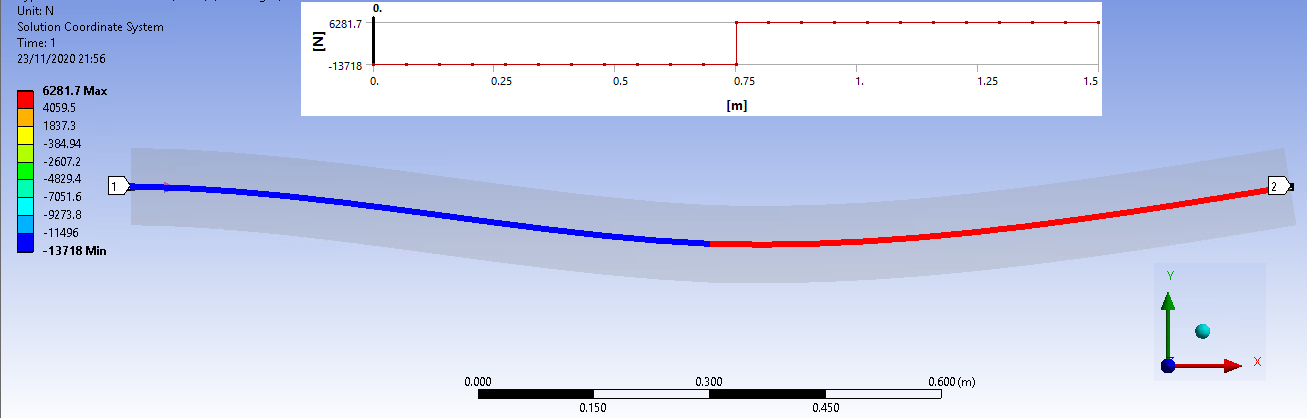
\includegraphics[width=\textwidth]{./img/DirectionalShearQ1.png}
    \caption{Directional shear in beam}
  \end{minipage}
  \hfill
  \begin{minipage}[b]{0.49\textwidth}
    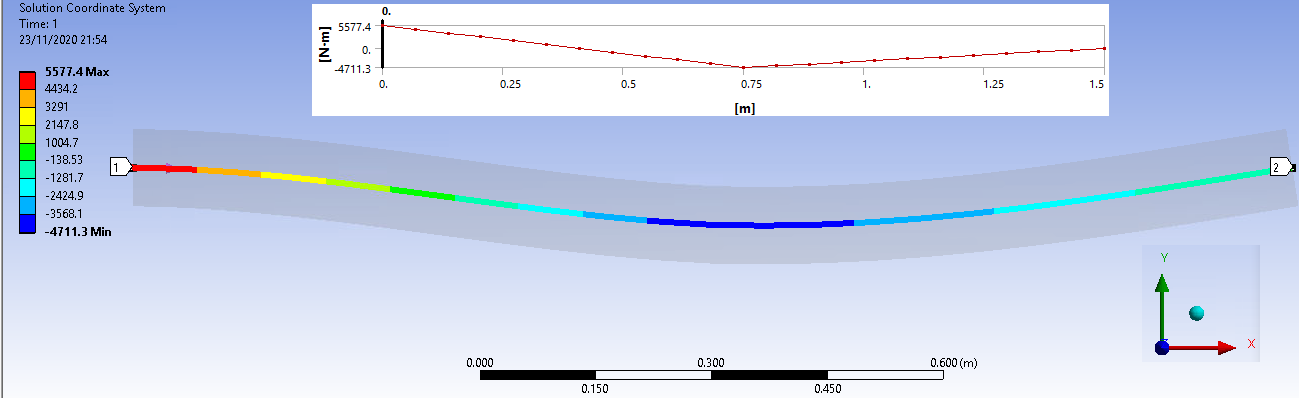
\includegraphics[width=\textwidth]{./img/DirectionalBendingQ1.png}
    \caption{Directional bending in beam}
  \end{minipage}
\end{figure}
\href{https://github.com/hashadar/ME-Latex/tree/master/MECH0013/Topic%20Notes}{FIX LINK} to see numerical data of the directional deformation and the bending moment of the beam. We can see that the beam bends in the middle with a rotation in the right side of the beam due to free rotation of the joint. This leads to a higher shear force and bending moment in the left side of the beam where it has a fixed support. We see that the maximum bending moment occurs at the fixed support. 
\section{Question 2}
\begin{figure}[H]
  \centering
  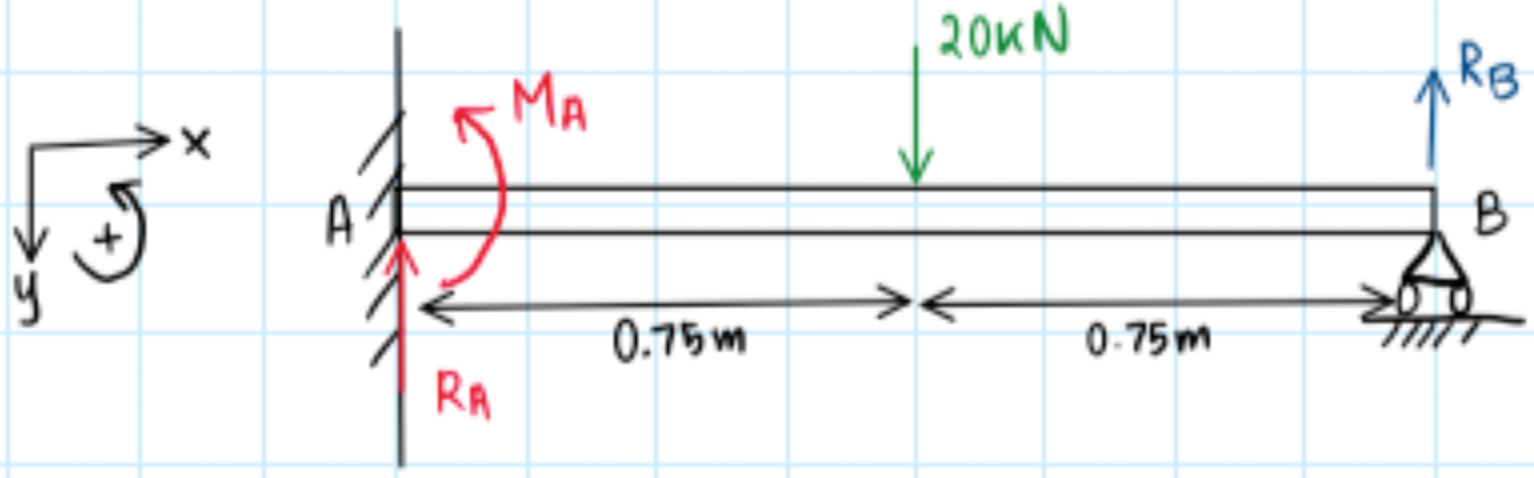
\includegraphics[width = 0.7\textwidth]{./img/Q1Sketch.png}
\end{figure}
\begin{align}
  \sum F_y = 0 \rightarrow &R_A + R_B = 20000 \label{Q1Eq1}\\
  \sum M_B = 0 \rightarrow &M_B + 20000(0.75) - R_A(1.5) = 0\\
  & M_A + 15000 - 1.5 R_A = 0 \label{Q1Eq2}
\end{align}
Determine second moment of area ($I$):
\begin{figure}[H]
  \centering
  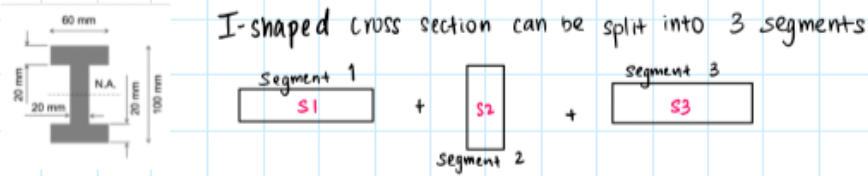
\includegraphics[width = 0.8\textwidth]{./img/SecondMomentOfInertiaQ2.png}
\end{figure}
Segment 1
\begin{align}
  I_x &= \bar{I}_x + Ady^2 = \frac{1}{12}(0.06)(0.02)^3 + (0.06)(0.02)(0.04)^2 = \SI{1.96e-6}{\meter\tothe{4}}
\end{align}
Segment 2
\begin{align}
  I_x &= \bar{I}_x + Ady^2 = \frac{1}{12}(0.06)(0.02)^3 + (0.06)(0.02)(0)^2 = \SI{3.6e-7}{\meter\tothe{4}}
\end{align}
Segment 3
\begin{align}
  I_x &= \bar{I}_x + Ady^2 = \frac{1}{12} (0.06)(0.02)^3 + (0.06)(0.02)(0.04)^2 = \SI{1.96e-6}{\meter\tothe{4}}\\
  I_{\textrm{total}} &= \SI{4.28e-6}{\meter\tothe{4}}
\end{align}
Macaulay's Method
\begin{align}
  M &= M_A + F(x-0.75) - R_A(x)\\
  \theta = -\frac{1}{EI} \int_{}^{} M \,\mathrm{d}x &= -\frac{1}{EI} \left[ M_A x + \frac{F(x-0.75)^2}{2} + \frac{R_A(x)^2}{2} \right] + \theta_0\\
  y = \int_{}^{} \theta \,\mathrm{d}x &= -\frac{1}{EI} \left[ \frac{M_Ax^2}{2} + \frac{F(x-0.75)^3}{6} + \frac{R_A (x)^3}{6} \right] + \theta_0 x + y_0
\end{align}
Boundary conditions. At $y= 0$, $x=0$:
\begin{align}
  y(0) = 0 = \theta_0 \cdot (0) + y_0 \rightarrow y_0 = 0
\end{align}
At $\theta = 0$, $x=0$:
\begin{align}
  \theta (0) = 0 = \theta_0 \rightarrow \theta_0 = 0  
\end{align}
At $y =0$, $x=1.5$:
\begin{align}
  y(1.5) &= 0 = -\frac{1}{EI} \left[ \frac{M_A(1.5)^2}{2} + \frac{F(1.5-0.75)^3}{6} + \frac{R_A (1.5)^3}{6} \right] + 0\cdot 1.5 + 0\\
  0 &= \frac{9}{8}M_A + 1406.25 - \frac{9}{16}R_A \label{Q1Eq3}
\end{align}
Multiply equation (\ref{Q1Eq2}) by $\frac{9}{8}$:
\begin{align}
  \frac{9}{8} M_A + 16875 - \frac{27}{16} R_A &= 0 \label{Q1Eq4}
\end{align}
Equations (\ref{Q1Eq4}) - (\ref{Q1Eq3}):
\begin{align}
  15468.75 = \frac{9}{8}R_A \rightarrow R_A &= \SI{13750}{\newton}\\
  \therefore M_A = 1.5(13750) - 15000 \rightarrow M_A &= \SI{5625}{\newton}\\
  \therefore R_B = 20000-13750 \rightarrow R_B &= \SI{6250}{\newton}
\end{align}
We know $y_{max}$ occurs at $\theta = 0$
\begin{gather}
  M_A x + \frac{F(x=0.75)^2}{2} - \frac{R_A x^2}{2} = 3125x^2 -9325x + 5625 = 0\\
  x\neq\SI{2.171}{\metre} \rightarrow x = \SI{0.829}{\metre} \ (3dp)\\
  y_{max} = -\frac{1}{EI} \left[ \frac{M_A(0.829)^2}{2} + \frac{F(0.829-0.75)^3}{6} + \frac{R_A (0.829)^3}{6} \right] = \SI{-2.099e-3}{\metre} \ (3dp)
\end{gather}
\begin{figure}[H]
  \centering
  \begin{minipage}[b]{0.49\textwidth}
    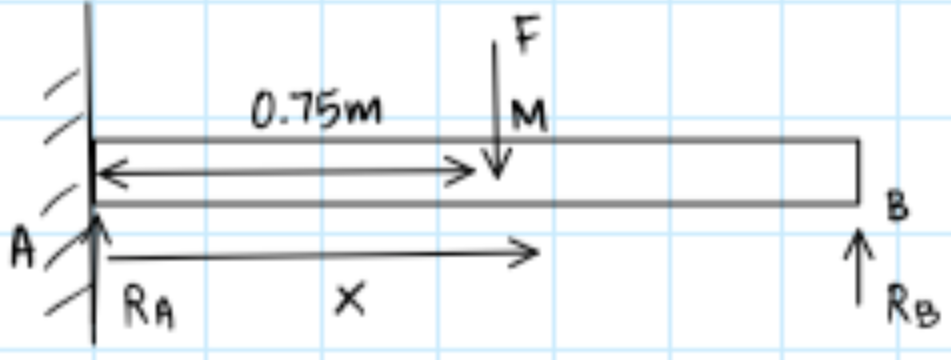
\includegraphics[width=\textwidth]{./img/Q2Sketch.png}
    \caption{Shear force diagram}
  \end{minipage}
  \hfill
  \begin{minipage}[b]{0.49\textwidth}
    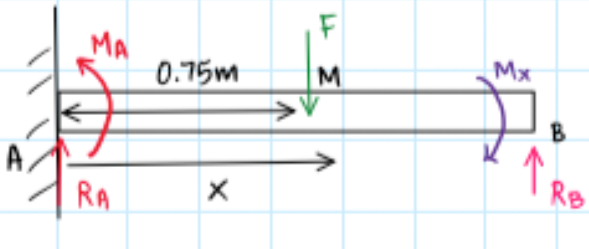
\includegraphics[width=\textwidth]{./img/Q2Sketch2.png}
    \caption{Bending moment diagram}
  \end{minipage}
\end{figure}
Section at $0 \leq x < 0.75$.
\begin{align}
  Q_x &= R_A = \SI{13750}{\newton}\\
  M_x &= M_A - R_A \cdot x = 5625 - 13750 x\\
\end{align}
Section at $0 \leq x < 1.5$.
\begin{align}
  \textrm{at } x &= 0, \ M_x = \SI{5626}{\newton\metre}\\
  \textrm{at } x &= 0.75, \ M_x = \SI{-4687.5}{\newton\metre}\\
  \textrm{at } x &= 1.5, \ M_x = \SI{0}{\newton\metre}
\end{align}
\begin{align}
  Q_x &= R_A - F = \SI{6250}{\newton}\\
  M_x &= M_A - R_A \cdot x + F(x - 0.75)\\
  M_x &= 5625 -13750x + 20000x - 15000\\
  M_x &= 6250x - 9375
\end{align}
\begin{figure}[H]
  \centering
  \begin{minipage}[b]{0.49\textwidth}
    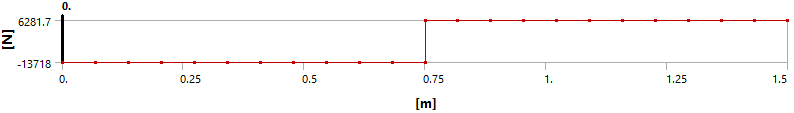
\includegraphics[width=\textwidth]{./img/Q2ShearAnsys.png}
    \caption{Ansys shear force graph}
  \end{minipage}
  \hfill
  \begin{minipage}[b]{0.49\textwidth}
    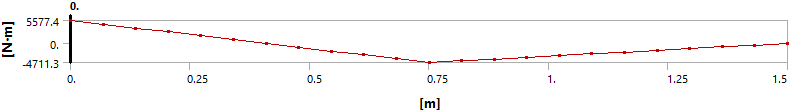
\includegraphics[width=\textwidth]{./img/Q2BendingAnsys.png}
    \caption{Ansys bending moment graph}
  \end{minipage}
\end{figure}
\begin{figure}[H]
  \centering
  \begin{minipage}[b]{0.49\textwidth}
    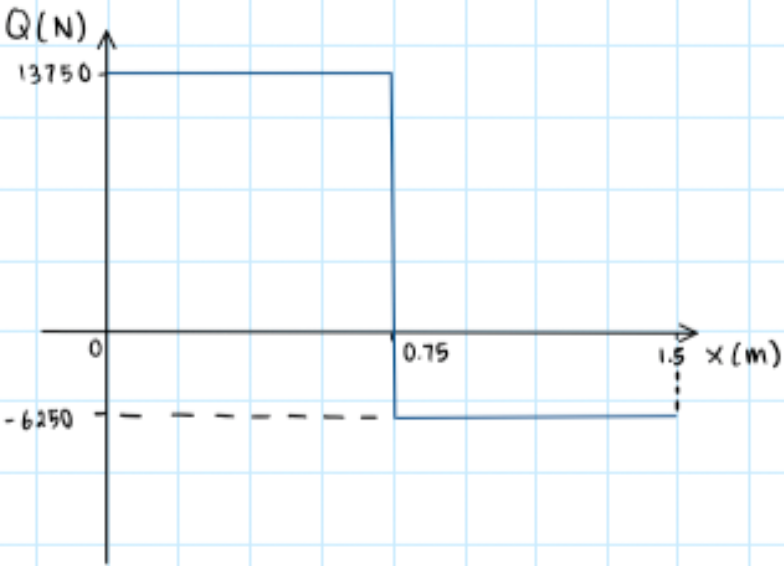
\includegraphics[width=\textwidth]{./img/Q2Shear.png}
    \caption{Shear force graph}
  \end{minipage}
  \hfill
  \begin{minipage}[b]{0.49\textwidth}
    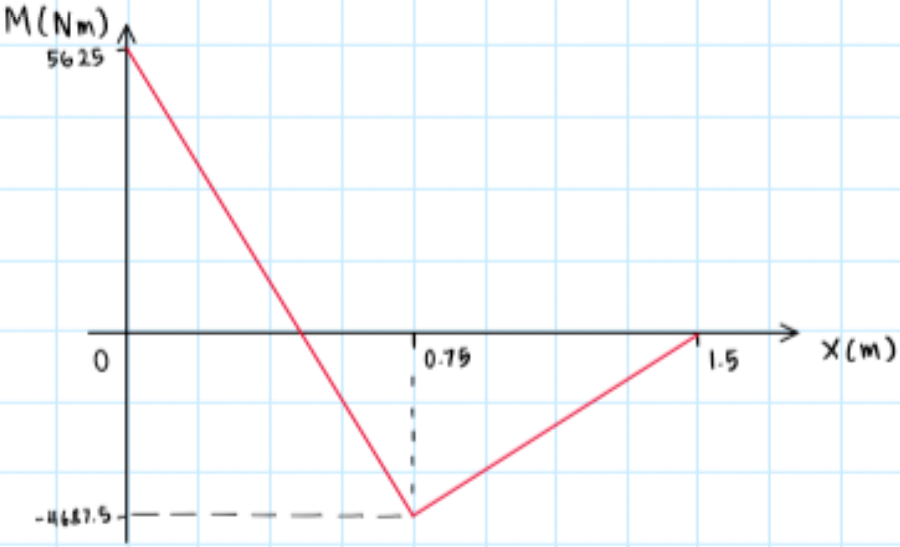
\includegraphics[width=\textwidth]{./img/Q2Bending.png}
    \caption{Bending moment graph}
  \end{minipage}
\end{figure}
\section{Question 3}
\begin{figure}[H]
  \centering
  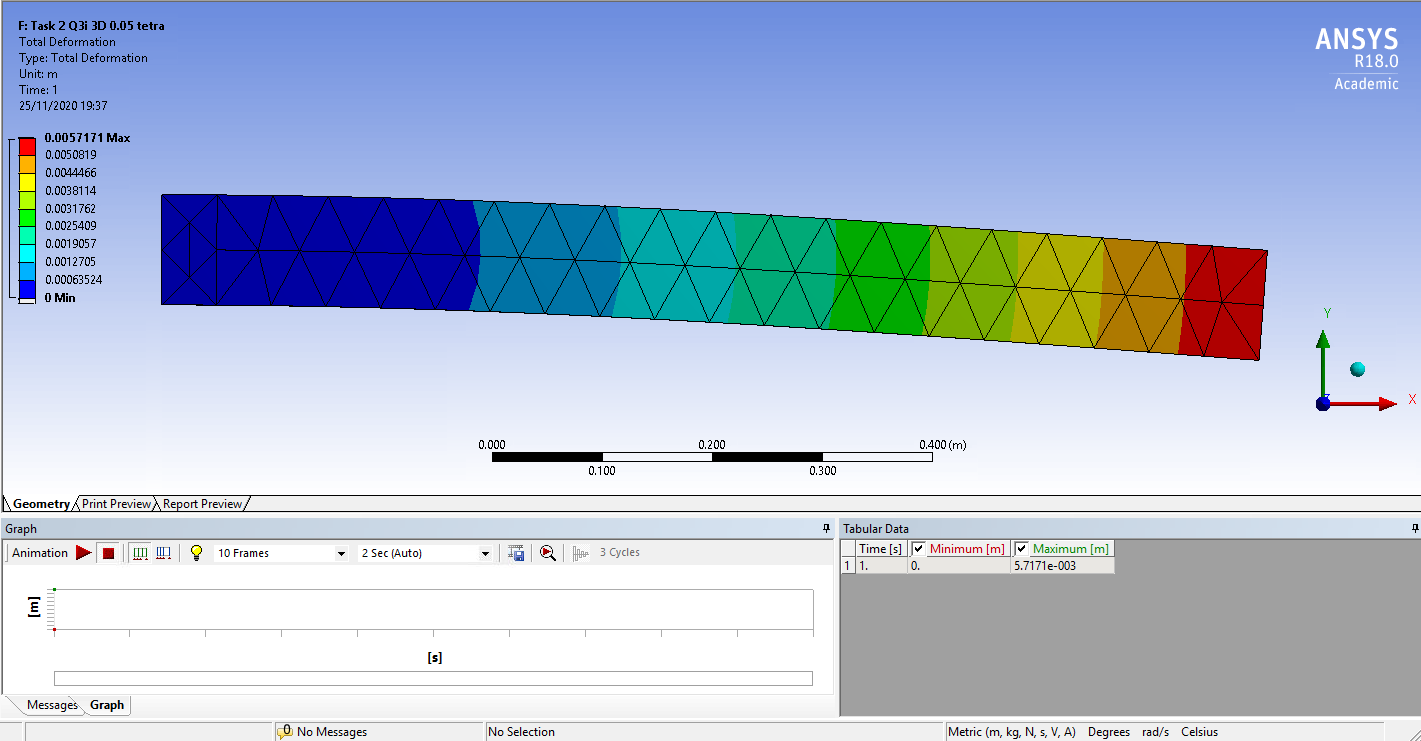
\includegraphics[width = 0.8\textwidth]{./img/Q3iDeformation.png}
  \caption{Tetrahedron mesh with size \SI{0.05}{\metre}}
\end{figure}
\begin{figure}[H]
  \centering
  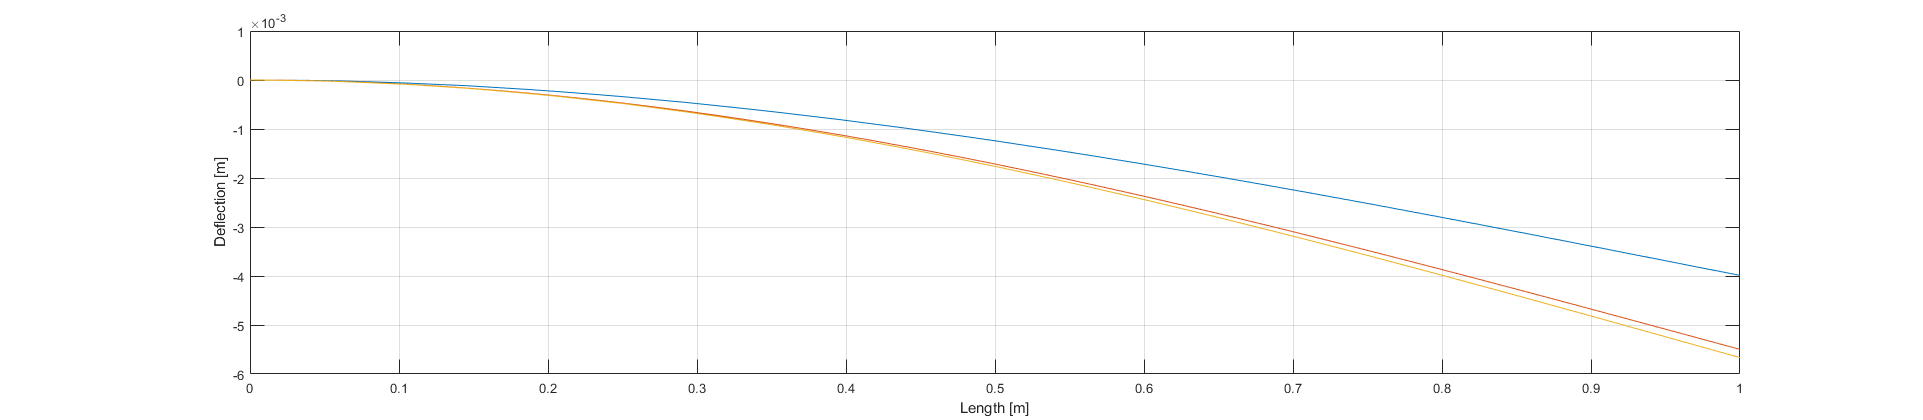
\includegraphics[width = 0.8\textwidth]{./img/q3graph.png}
  \caption{Tetrahedron mesh with size \SI{0.05}{\metre}}
\end{figure}
\section{Question 5}
\begin{figure}[H]
  \centering
  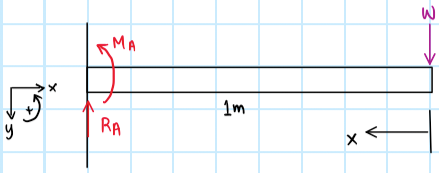
\includegraphics[width = 0.8\textwidth]{./img/Q3Analysis.png}
  \caption{Square section cantilever beam}
\end{figure}
Determination of support reactions:
\begin{align}
  \sum F_y = 0, \ R_A = w, \ R_A = \SI{1e4}{\kilo\newton}\\
  M_A = -w = \SI{-1e4}{\kilo\newton}
\end{align}
Determine second moment of area ($I$). Given a square cross-section:
\begin{align}
  I = \frac{BH^3}{12} = \frac{(0.1)(0.1)^3}{12} = \SI{8.33e-6}{\metre\tothe{4}}
\end{align}
Determination of deflection:
\begin{align}
  M &= wx\\
  \theta &= -\frac{1}{EI} \int M \dif x\\
  \theta &= -\frac{1}{EI} \left[ \frac{wx^2}{2} \right] + \theta_0\\
  y &= \int \theta \dif x\\
  y &= -\frac{1}{EI} \left[ \frac{wx^3}{6} \right] + \theta_0 x + y_0
\end{align}
Boundary conditions:
At $x = L$, $\theta = 0$:
\begin{align}
  0 = -\frac{wL^2}{2EI} + \theta_0 \rightarrow \theta_0 = \frac{wL^2}{2EI}
\end{align}
At $x = L$, $y = 0$:
\begin{align}
  0 = -\frac{wL^3}{6EI} + \frac{wL^3}{2EI} + y_0 \rightarrow y_0 = -\frac{wL^3}{3EI}
\end{align}
Thus,
\begin{align}
  \theta &= -\frac{1}{EI} \left[ \frac{wx^2}{2} \right] + \frac{wL^2}{2EI}\\
  y &= -\frac{1}{EI} \left[ \frac{wx^3}{6} \right] + \frac{wL^2}{2EI}x - \frac{wL^3}{3EI}
\end{align}
$y_{max}$ occurs at free end, $x = \SI{0}{\metre}$
\begin{align}
  y_{max} &= -\frac{1}{EI} \left[ \frac{w (0)^3}{6} \right] + \frac{wL^2}{2EI} (0) - \frac{wL^3}{3EI}\\
  y_{max} &= -\frac{wL^3}{3EI}\\
  y_{max} &= -\frac{10\times 10^{3} \times 1^3}{70 \times 10^9 \times 3 \times 8.33 \times 10^{-6}}\\
  y_{max} &= \SI{-5.714e-3}{\metre}
\end{align}
\end{document}